\subsection{Combustion Instabilities in Liquid-propellant Rocket Engines}

In the 21st century, the ability to launch objects into space is critical to the function of national governments, corporations, and scientific research organizations alike. Space is now increasingly accessible to developing countries and inseparable from the everyday lives of people around the world. The impact of space vehicles, probes, and satellites is experienced in both mundane tasks and life-critical operations. Communication satellites provide data transmission for cell phones, and GPS satellites provide real-time location and navigation services. Cameras pointed at the Earth from satellites help track storms and wildfires and allow us to observe dangers to the environment as glaciers recede and rainforests are cut. Space stations provide a testing ground for life to thrive beyond Earth, and enable new discoveries in medicine, agriculture, and engineering to improve life on Earth. Space telescopes peer into the depths of the universe to help us better understand our place in the cosmic soup of galaxies, suns, and planets. These extra-planetary objects accomplish incredible things, and getting them into space requires similarly incredible feats of engineering.

Launching these massive objects (many satellites weigh over one ton) into space is accomplished exclusively by chemical rocket propulsion. No other practical means of propulsion is able to generate the force required to lift payloads hundreds of miles and reach velocities greater than 15,000 miles per hour. Rocket engines accomplish this by reacting chemicals which generate high-temperature and high-pressure gases in a combustion chamber, forcing these gases through a nozzle which accelerates them to supersonic speeds, and then ejecting the gases behind the engine. This ejection of high-speed gas imparts enormous force, or thrust, on the rocket: the nine Merlin 1D engines of the SpaceX Falcon rocket impart 1.71 million pounds-force (7.686 MN) of thrust~\cite{falconGuide}. Figure~\ref{fig:tcCrossSec} illustrates these elements of the thrust chamber. While air-breathing jet engines, like those which power commercial aircraft or military fighter planes, are capable of generating moderate thrust levels (the General Eletric GEnx-1B76 can generate over 76 thousand pounds-force, or 339 kN~\cite{genxSpecs}), they ultimately suffer from an unfortunate lack of air in space.

Chemical rocket propulsion comes in two dominant forms: solid and liquid propellants. Solid propellants are composed of combustible reactants cured into a solid fuel grain. When fired, it sustains a highly-energetic reaction converting solid fuel into hot gases until the entire grain is consumed. Solid rocket motors can be stored at room temperature for long periods of time, can be ignited instantly, and require few to no auxiliary systems to operate. As such, they play a dominant role in rocket-propelled munitions such as rocket artillery and missiles, like the American LGM-30 Minuteman intercontinental ballistic missile. However, solid propellant reactions are extremely difficult to control, as combustion cannot be stopped once it begins. Further, the reaction of solid propellants tends to be far less efficient than reactions between many liquid or gaseous propellants, achieving lower specific impulse values~\cite{Sutton2003}.

Due to the limitations of solid propellants, liquid propellants are, by far, the preferred method to power space launch vehicles. They enable much more fine-tuned thrust control: liquid engines have been designed to shut down and restart multiple times (e.g., the Apollo Lunar Module reaction control system), and the thrust can be actively throttled to adjust the rocket's trajectory (e.g., SpaceX Falcon purported to throttle down to $\sim$25\% of maximum thrust). There are two primary variants of liquid propellants: bipropellants and monopropellants. Bipropellants involve a liquid oxidizer (e.g. oxygen, dinitrogen tetroxide) and liquid fuel (e.g., hydrogen, kerosene, monomethylhydrazine), which are mixed and atomized into a gas before combustion. Monopropellants involve a single propellant (e.g., hydrazine) which decomposes in a highly exothermic reaction when it comes in contact with a catalyst. The selection of liquid propellants largely depends on the engine's mission (e.g., launch, station-keeping, orientation control) and a balance of combustion efficiency (liquid hydrogen and oxygen is the most efficient), cost (kerosene is cheaper than hydrogen to manufacture and store~\cite{propellantCosts}), and safety risk (monomethylhydrazine is highly toxic). In this thesis, we will only examine systems of non-hypergolic bipropellants.

\begin{figure}
	\begin{minipage}{0.48\linewidth}
		\centering
		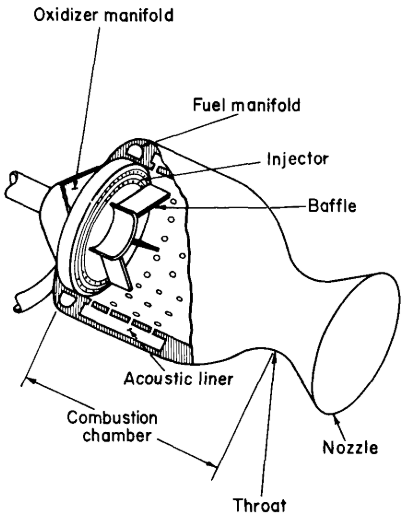
\includegraphics[width=0.61\linewidth]{Chapters/Overview/Images/nasa_thrust_chamber_cross_sec.png}
		\caption{\label{fig:tcCrossSec}Cross section of liquid bipropellant thrust chamber (NASA~\cite{NASA1972}).}
	\end{minipage}
	\hspace{1em}
	\begin{minipage}{0.48\linewidth}
		\centering
		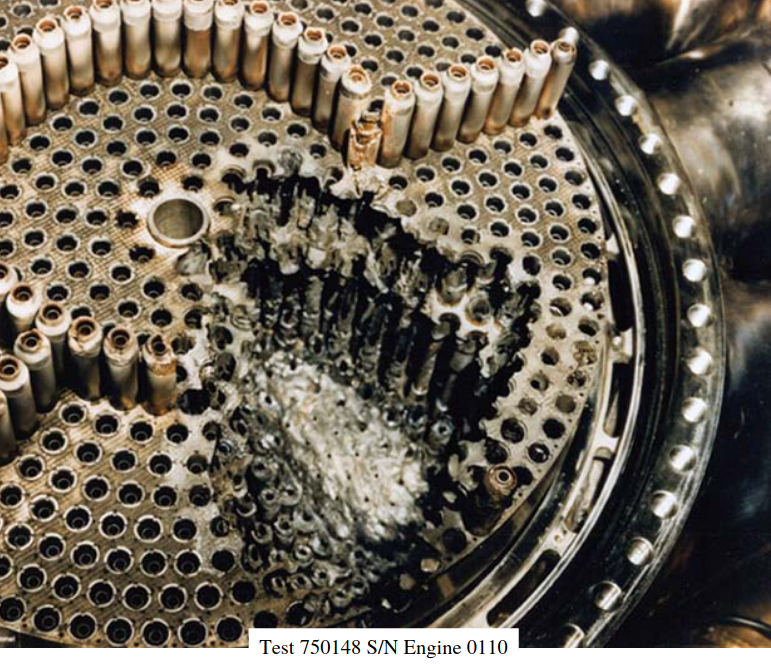
\includegraphics[width=0.9\linewidth]{Chapters/Overview/Images/ssmi_failure_border.png}
		\caption{\label{fig:ssmiFailure}Failure of Space Shuttle main injector assembly (Goetz and Monk, NASA~\cite{Goetz2003}).}
	\end{minipage}
\end{figure}

Despite many benefits, the design, manufacturing, and operation of liquid propellant rocket engines are not without major complications. They require complex pump systems to pressurize the propellants and intricate injection systems to mix and atomize the liquid to promote efficient combustion. Further, some propellants must be stored at temperatures below -400 $^{\circ}$F (-240 $^{\circ}$C)~\cite{liquidHydrogenProps}. Even leveraging extensive engineering design practices honed over decades of rocket engine development programs, producing a successful engine is a dangerous process requiring frequent testing and rigorous certification. One design flaw which has troubled engine designers for decades is the possibility of \textit{combustion instabilities}.

Combustion instability broadly refers to organized vibrations in the liquid propellants, combustion gases, or solid structure which can degrade engine performance, and potentially damage or complete destroy the engine. There are three general categories of such instabilities: propellant feed instabilities (``chugging''), intermediate instabilities (``buzzing''), and resonant combustion (``screaming''). As these colloquial names may imply, these are listed in order of increasing frequency of the vibration and relative danger to the integrity of the engine. Chugging instabilities are low-frequency, low-amplitude oscillations generated by irregular injection of propellants, leading to the accumulation of unburnt reactants and subsequent explosive reaction. Buzzing instabilities often result from the intermediate-frequency coupling of acoustic waves in the reacting gases and the structural components of the engine assembly. Chugging and buzzing are not always a threat to the engine's integrity, but can lead to decreased, irregular performance.

The final instability, screaming, refers to a highly destructive feedback mechanism between acoustic waves in the combustion chamber and the unsteady heat release caused by the reaction of the propellants. The reaction generates heat, which raises the pressure of the reacting gases, which in turn encourages a more vigorous reaction, which generates more heat, and so on. Depending on the geometry of the combustion chamber, the composition, temperature, and flow rate of the propellants, and the ability of the engine's structure to dissipate acoustic energy, this feedback loop may amplify the acoustic waves to enormous amplitudes. The intensity of this process is illustrated by CH* chemiluminescence images captured by Orth \textit{et al.}~\cite{Orth2018}, displaying the immense difference in heat release in a rocket combustor without and with unstable combustion. These large pressure waves and the accompanying high heat-release rates may shake the engine apart, or burn through the combustion chamber walls or propellant injection mechanisms. An example is shown in Fig.~\ref{fig:ssmiFailure}, where vibrations in the Space Shuttle main engine cracked oxidizer injectors and burned through the injector face, to catastrophic effect. Unlike chugging and buzzing, which can often be accommodated for or easily fixed, screaming is nearly impossible to predict and there exist no sure methods of preventing it. Many possible mechanisms have been proposed as the cause of high-frequency combustion instabilities, but the extreme complexity of the system (multi-phase, high-pressure, turbulent combustion) has eluded any strong consensus on the topic.

\begin{figure}
	\begin{minipage}{0.49\linewidth}
		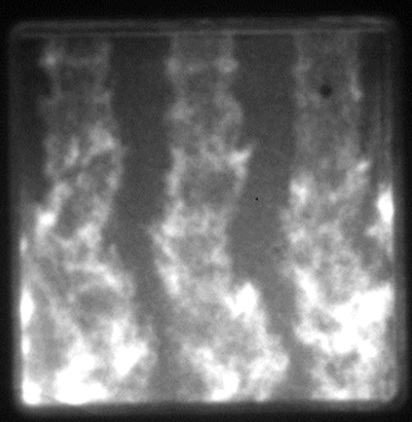
\includegraphics[width=0.98\linewidth]{Chapters/Overview/Images/orth_chChem_stable.png}
	\end{minipage}
	\begin{minipage}{0.49\linewidth}
		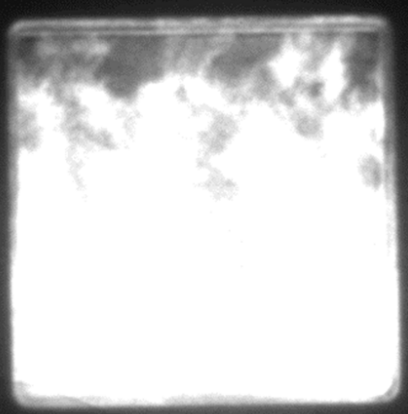
\includegraphics[width=0.99\linewidth]{Chapters/Overview/Images/orth_chChem_unstable.png}
	\end{minipage}
	\caption{\label{fig:orthCombustor} CH* chemiluminescence photos of multi-element rocket combustor in stable combustion (left) and unstable combustion (right) (reproduced with permission from~\cite{Orth2018}) \textcolor{red}{I have not received permission yet}}
\end{figure}

Screaming has been catalogued in engine development dating back to the 1950's in the American Thor and Atlas missile programs, and continued to plague development programs throughout the prolific USA-USSR Space Race era and beyond. A classic example of an extreme engineering challenge caused by combustion instabilities is the development of the Rocketdyne F-1 engine, which to this date remains the most powerful American liquid-propellant engine to launch. In the early stages of its development, almost every single engine test ended abruptly with the onset of dangerous combustion instabilities. What proceeded was the long, arduous Project First program, assembled to eliminate sustained combustion instabilities, lasting from October 1962 until the flight certification of the propellant injector in November 1965~\cite{Young2008}. The program amounted to iterative modifications to propellant spray patterns (e.g., increasing the spray impingement distance), propellant injector port arrangements, and patterns of metal baffles between sections of the injector plate. Illustrations of such baffles can be seen in Fig.~\ref{fig:tcCrossSec}. Many of these tests failed to eliminate combustion instabilities, and the program ultimately accounted for approximately 2,000 of the $\sim$3,000 full-scale engine tests~\cite{Oefelein1993}. Although the project was ultimately a success, it was an extremely labor- and time-intensive effort. To this day, similar iterative, \textit{ad hoc} approaches remain the preferred method of eliminating combustion instabilities. Although advances have been made in the construction of acoustic dampers~\cite{Zhao2015}, they are not a guaranteed solution.

A number of analytical methods have been formulated in attempts to predict the onset of sustained high-frequency combustion instabilities and avoid costly experimental campaigns. However, due to the extremely non-linear physics of coupled combustion and fluid flow dynamics, paired with the complex geometry and propellant injection configurations in rocket engines, these methods often rely on linearizations or oversimplifications of the rocket engine physics. They are often incapable of incorporating the effects of possible damping mechanisms such as baffles and acoustic liners, or possible driving mechanisms such as irregular distribution of propellants~\cite{Yang1995}. Further, those methods which do yield accurate predictions of instabilities are usually valid for relatively small-amplitude acoustic waves or unable to predict a limit cycle~\cite{Culick1994}. Although significant effort has been taken to develop accurate models for gas turbine combustors in recent decades (e.g.,~\cite{Noiray2008}), the contemporary analytical combustion instability theory for rocket combustors is comparably lacking.

In the modern era, in which private companies such as Blue Origin, SpaceX, Boeing, and Lockheed Martin vie for a lucrative heavy-launch market and NASA takes a relative back seat, publicly-available data on engine development programs is scarce. However, there have been occasional hints that combustion instabilities continue to haunt engine design programs well into the 2020's~\cite{blueOriginTweet}. With the understanding that analytical methods of predicting instability fall short in their generalizability, and extensive test campaigns may incur excessive costs, we now turn to the use of numerical simulations in the modeling of reacting fluid flows, with an emphasis on applications to rocket combustors.
